\documentclass[15pt,a4paper,oneside,openright]{report}
\usepackage[greek,english]{babel}
\usepackage[iso-8859-7]{inputenc}
\usepackage[margin=3cm]{geometry}
\usepackage{fancyhdr}
\usepackage{graphicx}
\usepackage{caption}
\usepackage{subcaption} 
\usepackage{makeidx}
\usepackage{float}
\usepackage[cc]{titlepic}
\usepackage{amsmath}
\usepackage{mathabx}
\usepackage{wrapfig}
\usepackage{titletoc}
\usepackage{array}
\usepackage{enumitem}
\usepackage{enumerate}
\usepackage[colorlinks=true,linkcolor=blue]{hyperref}
\newcommand{\HRule}{\rule{\linewidth}{0.5mm}}
\renewcommand{\familydefault}{\sfdefault}

\pagestyle{fancy}
\setlength{\parindent}{0cm}

\usepackage[absolute]{textpos}

\begin{document}

\begin{titlepage}
\begin{center}

\begin{textblock*}{297mm}(-44mm,0mm)
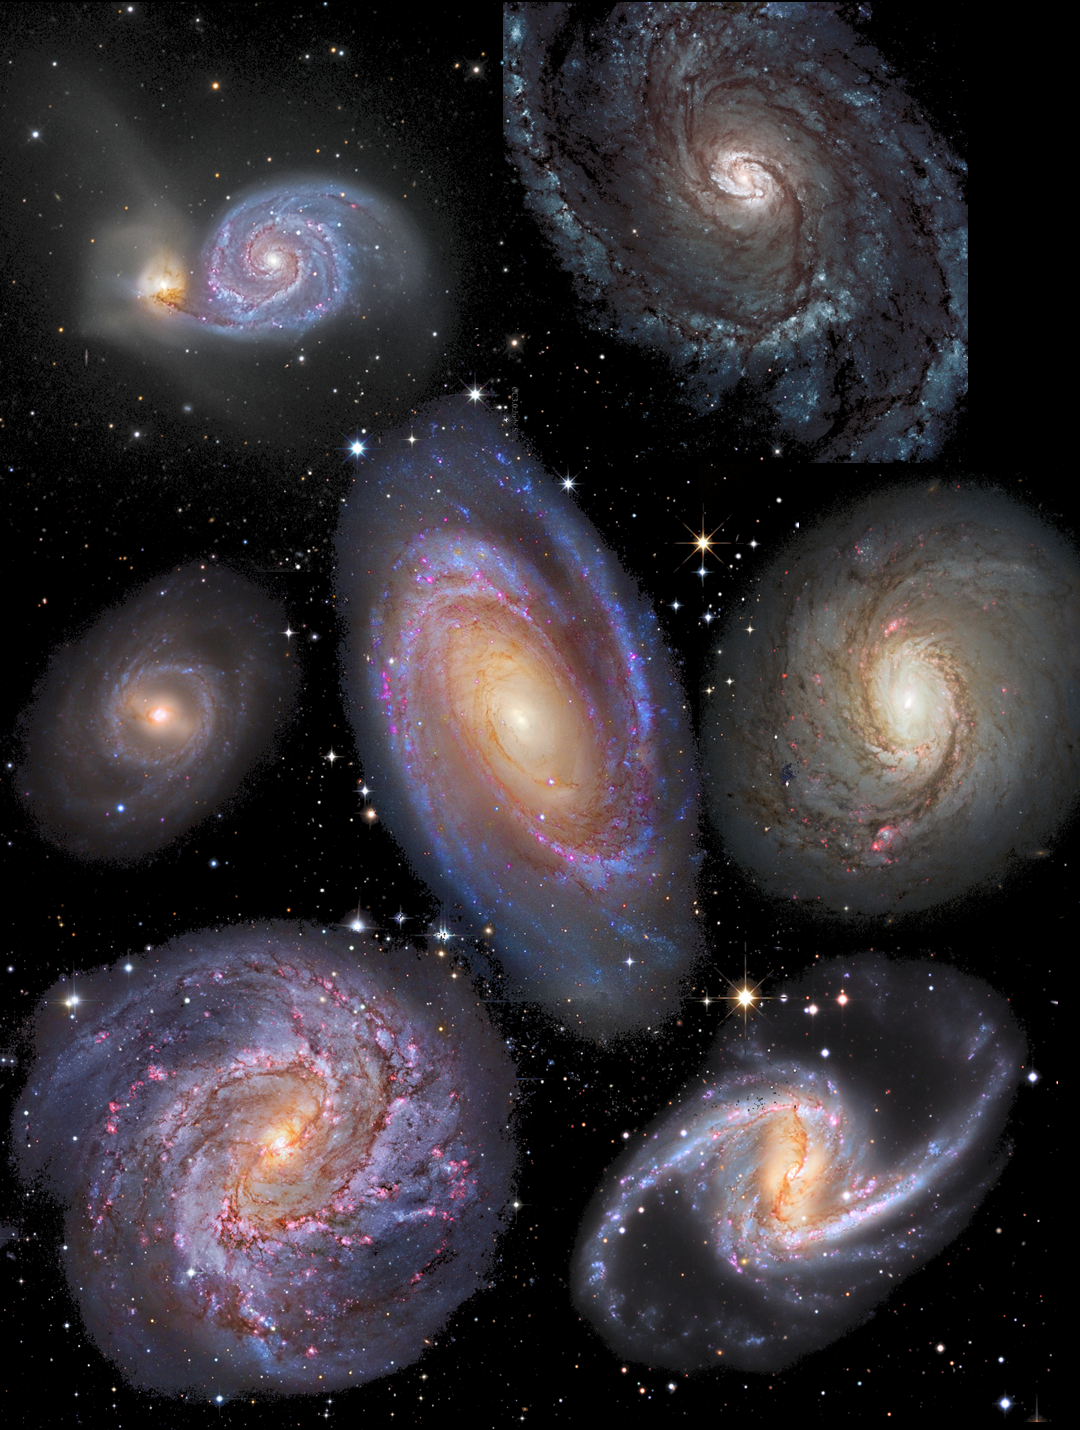
\includegraphics[scale=1.]{figures/galaxies_rotated.png}
\end{textblock*}

{\color{white}\HRule \\[0.3cm]}
\textcolor{white}{\huge \bfseries PTS/Modeling: \\ A User Friendly Guide}\\[0.3cm]
{\color{white}\HRule \\[0.3cm]}

\vspace{3.0cm}
\textcolor{white}{\textsc{\Large Ghent University, 2018}\\[1.5cm]}

%\textsc{\Large Department of Physics}\\[0.5cm]
%\includegraphics[width=1.0\textwidth]{figures/galaxies.png}\\[0.5cm] 
%\textsc{\large}\\[0.5cm] 

\vfill 
\textcolor{white}{\textsc{\large Angelos Nersesian\\Sam Verstocken}\\[0.5cm]}

%\textsc{\large UGent 2018}\\[0.5cm]
%\includegraphics[width=0.80\textwidth]{galaxies.png}\\[0.5cm] 

\end{center} 
\end{titlepage}

\subsubsection{Greetings}

\vspace{10mm}

Dag! Welcome to the awesome world of galaxy modeling with PTS. PTS (\textbf{P}ython \textbf{T}oolkit for \textbf{S}KIRT) 
is a python based code that helps the user to setup the modeling environment as well to process 
the galaxy images and create the necessary components for the simulations with SKIRT. It is assumed that you have already installed PTS on your local PC environment and preferably to a remote computer as well. If this is not the case, then click this \href{http://www.skirt.ugent.be/pts/index.html}{link} to go to the installation page. \textbf{Caution}; PTS works with \textbf{Python-2.7.0}, thus it is also best to install \href{https://anaconda.org/anaconda/python}{Anaconda}, which allows the user to switch between different python environments. I hope this manual serve you well in your journey. Enjoy!

\tableofcontents

\part{Preparing PTS}

Create a new host with:\\

\textbf{\$ pts configure\_host}\\

View the required packages:\\

\textbf{\$ pts depends model}\\

Will give the following output:

\begin{center}
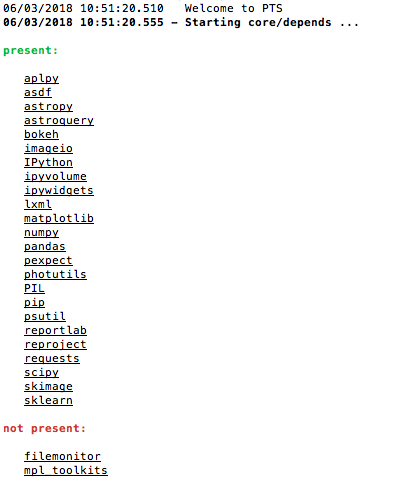
\includegraphics[width=0.5\textwidth]{figures/depends.png}
\end{center}

Install the required packages manually or use\\

\textbf{\$ pts install\_pts},\\

and it will install of its dependencies (all those listed with \textbf{pts depends} without command).\\

Install SKIRT locally and remotely:\\

\textbf{\$ pts install\_skirt}\\
\textbf{\$ pts install\_skirt [host\_id]}\\

Optionally, you can also already deploy PTS on one or multiple remotes (you will probably need it, depending on the capabilities of your own computer), using:\\

\textbf{\$ pts install\_pts [host\_id]}\\

Yes, it's as simple as that.

\begin{center}
\textbf{CONTINUED IN PART II...}
\end{center}

\part{Setting Up Your Modeling Environment}

%\chapter{Setup}

Open a new terminal in your home directory (or anywhere else that you like), and create a new folder (e.g. hres\_3drtm).\\

\textbf{\$ mkdir [hres\_3drtm]}\\

\textbf{\$ cd [hres\_3drtm]}\\

\textbf{\$ pts setup}\\

A prompt window will open asking you for the setup info. Use the following values 
when you asked. When there is a prompt that it's not included below just press enter
to use the default value.

\begin{itemize}
	\item Type of modeling: [2] galaxy: 3D model
	\item Name: 'Give the name of your galaxy'
	\item Fitting method: [1] grid
	\item Fitting host ids: "Choose one of the available remote computers"
	\item Modeling method: [0] De Looze et al. 2014
\end{itemize}

A new directory was created named after your galaxy (ex. NGC3351/M95). This is the \textbf{modeling} directory.\\

\textbf{\$ cd [M95]}\\

This directory includes all necessary folders where your data will be saved, named after the different stages of the modeling. 
In addition to the different directories, three files exist, each one of them containing information about your modeling progress.

\begin{itemize}
	\item commands.txt
	\item history.dat
	\item modeling.cfg
\end{itemize}
 
In "commands.txt" all the executed commands are saved.\\

In "history.dat" the status of your work is saved.\\  

In "modeling.cfg" you can check your setup configuration and modify it if you want.\\

PTS is written in such a way that you can process your images step by step or automated. If you execute the command:\\

%\chapter{Model}

\textbf{\$ pts model}\\

PTS will start running automatically all the following commands stopping only when a bug occurs or when there is a deliberate User Intervention
to check the images. However, it is recommended to do the image process step by step so that you can have full control of your
actions and check continuously the output and make changes when necessary.\\

The first command collects the general properties of your galaxy.\\

\textbf{\$ pts fetch\_properties}\\

Get the SEDs from different catalogs.\\ 

\textbf{\$ pts fetch\_seds}\\

The following catalogs are recommended:

\begin{itemize}
	\item $\left[0\right]$ DustPedia\footnote{If your galaxy is included in the DustPedia database, 
	\href{http://dustpedia.astro.noa.gr/}{http://dustpedia.astro.noa.gr/}.}
	\item $\left[1\right]$ GALEX
	\item $\left[2\right]$ 2MASS
	\item $\left[4\right]$ LVL
	\item $\left[5\right]$ Spitzer
	\item $\left[7\right]$ IRAS
	\item $\left[8\right]$ IRAS/FSC
	\item $\left[9\right]$ S4G
\end{itemize}

Next command downloads all available images of your galaxy. A prompt window will open asking you stuff. 
One of the options is to create the error maps for GALEX and SDSS bands. It is highly recommended
to create the error maps separately. So decline politely when you were asked.\\

\textbf{\$ pts fetch\_images}\\

The images are saved in "/data/images/". When the download of the images is complete you can create the poisson error maps. 
Create a new folder inside the \textbf{modeling} directory.\\

\textbf{\$ mkdir make\_galex}\\

\textbf{\$ cd make\_galex}\\

The following command will download the mosaics of your galaxy from the GALEX database and will make the 
poisson error maps. A prompt window will open; select all default options. When you asked about how many 
\textbf{number of processes} to use, the default option is \textbf{8}. If you run this command in a \textbf{local PC} it is recommended 
to select \textbf{1} instead of 8.\\

\textbf{\$ pts make\_galex}\\

The results will be in the "out/" directory. Change the name of the image; for example, 
"NGC3351\_GALEX\_FUV\_errors.fits" to "NGC3351\_GALEX\_FUV\_poisson.fits", and move the following files to "/data/images/GALEX/". 
Before you move these files, make sure to move the existing GALEX images in "/data/images/GALEX/" to a different directory. For example, 
create a new directory in "/data/images/GALEX/" called "/temp" and move your images there.

\begin{itemize}
	\item "NGC3351\_GALEX\_FUV.fits"
	\item "NGC3351\_GALEX\_FUV\_poisson.fits"
	\item "NGC3351\_GALEX\_NUV.fits"
	\item "NGC3351\_GALEX\_NUV\_poisson.fits"
\end{itemize}

Follow the same steps for the SDSS error maps. Go back to the \textbf{modeling} directory and type:\\

\textbf{\$ mkdir make\_sdss}\\

\textbf{\$ cd make\_sdss}\\

\textbf{\$ pts make\_sdss}\\

At this point, search for an H${\alpha}$\footnote{The H${\alpha}$ image must be continuum subtracted.} image of your galaxy on NED\footnote{\href{http://ned.ipac.caltech.edu/}{http://ned.ipac.caltech.edu/}} or other databases. Also, make sure that you have images in the optical bands, SDSS (u,g,r,i,z). 
It is important for the modeling procedure to have at least an image in the R-band. If your galaxy does not have SDSS data, search on NED for an R-band 
image. Furthermore, read the "High-resolution 3D radiative transfer model guidelines" to check which images are necessary for the galaxy modeling and 
what to do when you are missing images, such as SDSS\_r, Spitzer\_3.6 or H${\alpha}$.\\

After you download the images from NED, check the units of the images and convert, if necessary, the image units to Jy and the H${\alpha}$ image units to erg/sec. Move the images to the appropriate folders in the "/data/images/" directory.\\

\textbf{TIP!}/ Name the R image as "NGC3351\_SDSS\_r.fits" and move it to the "SDSS" folder.\\

This step is not mandatory, but you can inspect one by one your images and try to mask some of the very bright sources around your galaxy. Check images 
like GALEX (FUV, NUV), SDSS (u, g, r, i, z), H$\alpha$, IRAC (I1, I2, I3, I4, MIPS24) and WISE (W1, W2, W3, W4). 
Open the images with ds9, select the sources to be masked and create a region file in the same directory as your image (select, Coordinate System: image). 
Navigate to the appropriate directory where your image and region file are and type:\\

\textbf{\$ pts interpolate [NGC3351\_Halpha.fits ds9.reg] -o out -{}-debug}\\

This command will mask the selected sources and will interpolate the selected regions. The "out/" directory includes the new image and the mask. 
Rename your original image as "NGC3351\_Halpha\_original.fits" and move it along with the region file to the "out/" directory. Move the 
interpolated image "NGC3351\_Halpha.fits" to the original image directory.

\begin{center}
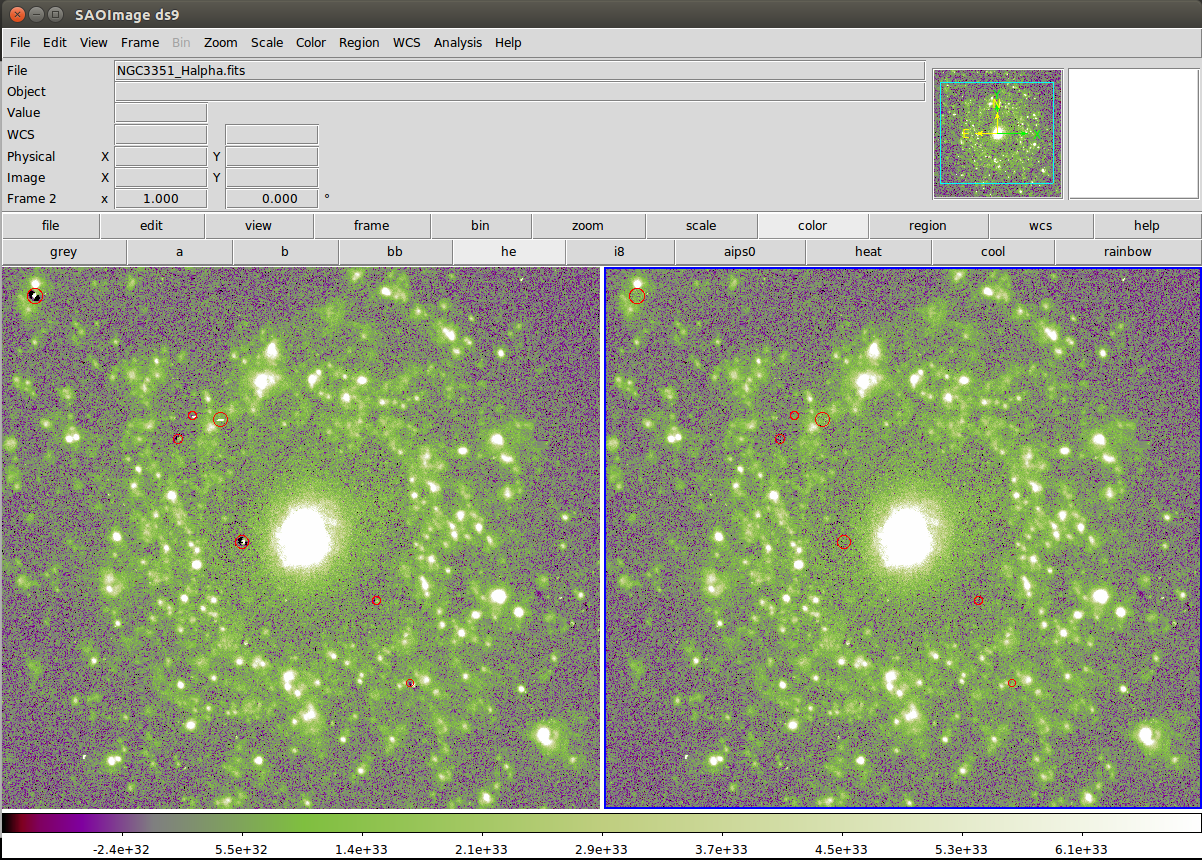
\includegraphics[width=0.8\textwidth]{figures/pts_interpolate_halpha.png} 
\end{center}

To complete this part, you need to inspect the information that is written in the headers of your images. Go to the \textbf{modeling} directory
and type:\\

\textbf{\$ pts inspect\_data}\\

This command inspects the headers of all images and creates a plot with their coordinate ranges.
Check the plot in the "/inspect/inspect\_data/" directory.\\

\begin{center}
\textbf{CONTINUED IN PART III...}
\end{center}

\part{Prepare Your Images}

Let's start now with the most intriguing and most demanding part of the whole project. In this Part, we will detect and extract the sources (stars, galaxies) from the images, correct them for galactic extinction, subtract the sky and create the error-maps.\\

For this step, we will use the \textbf{\$ pts model} command because it raises a User Intervention error at the very end. Furthermore, for the rest of
the guide, it is recommended to use \textbf{-{}-debug} at the end of each command, while you can always type the name of the command and \textbf{-{}-help}
so that you can get all the available argument that you can use for that specific command.\\

Start the initialization process by typing:\\

\textbf{\$ pts model -{}-debug -{}-local -{}-nprocesses 1}\\

This command will initialize the data preparation. The options -{}-local and -{}-nprocesses 1 used to run the initialization in your local PC.
This command will create an initialization image for each band, in the "prep/" directory and it will detect all sources in your images, and create two catalogs one for the extended sources and one for the point sources. Then, the User Intervention message will be printed and PTS will stop.\\

Check your images and the region files within the directory "prep/Band\_Name/sources" with ds9. Make sure that the program didn't confused areas of your galaxy 
as stars. Load first the region file "stars.reg". If there are green or blue circles on top of your galaxy and you are sure that they are not stars remove 
the circles and save the new region file. Then load the region file "saturation.reg". If there are white ellipses/circles on top of your galaxy remove them. Do this exercise for all bands. For the H$\alpha$ image load the "other\_sources.reg" and make sure that none of the galaxy regions is selected.\\

When you finish the data inspection, you can start the image processing by typing:\\

\textbf{\$ pts prepare\_data -{}-debug}\\

This command will go through all your images automatically and extract the detected sources around your galaxy, will correct the images for extinction\footnote{Images will be corrected for extinction in the wavelength range, $0.005-10 \ \mu m$.}, it will estimate subtract the sky background and finally will create the error-maps 
by adding quadratically the poisson errors\footnote{Poisson errors are only available for the GALEX and SDSS images.}, the calibration errors and the sky errors.\\

However, by using the automated way means that you will use all the default values that might not suit best your galaxy. Thus it is recommended to prepare each image independently and inspect every step of the image processing carefully. For example, inspect if the source extraction was done properly. Open 
the "extracted.fits" and confirm that everything looks fine (check for long white lines or boxes that might cross your galaxy). To do that type:\\    

\textbf{\$ pts prepare\_data [Band\_Name] -{}-debug -{}-annulus\_inner\_factor 1.2 -{}-annulus\_outer\_factor 4.0 -{}-sky\_estimation\_method photutils -{}-interactive\_sky}\\

All options in the previous command are related to the sky subtraction method. The sky subtraction is the most important step in this stage and demands extra care 
from the user. The \textbf{-{}-interactive\_sky} option helps you to visualize the annulus ellipses.\\ 

\begin{center}
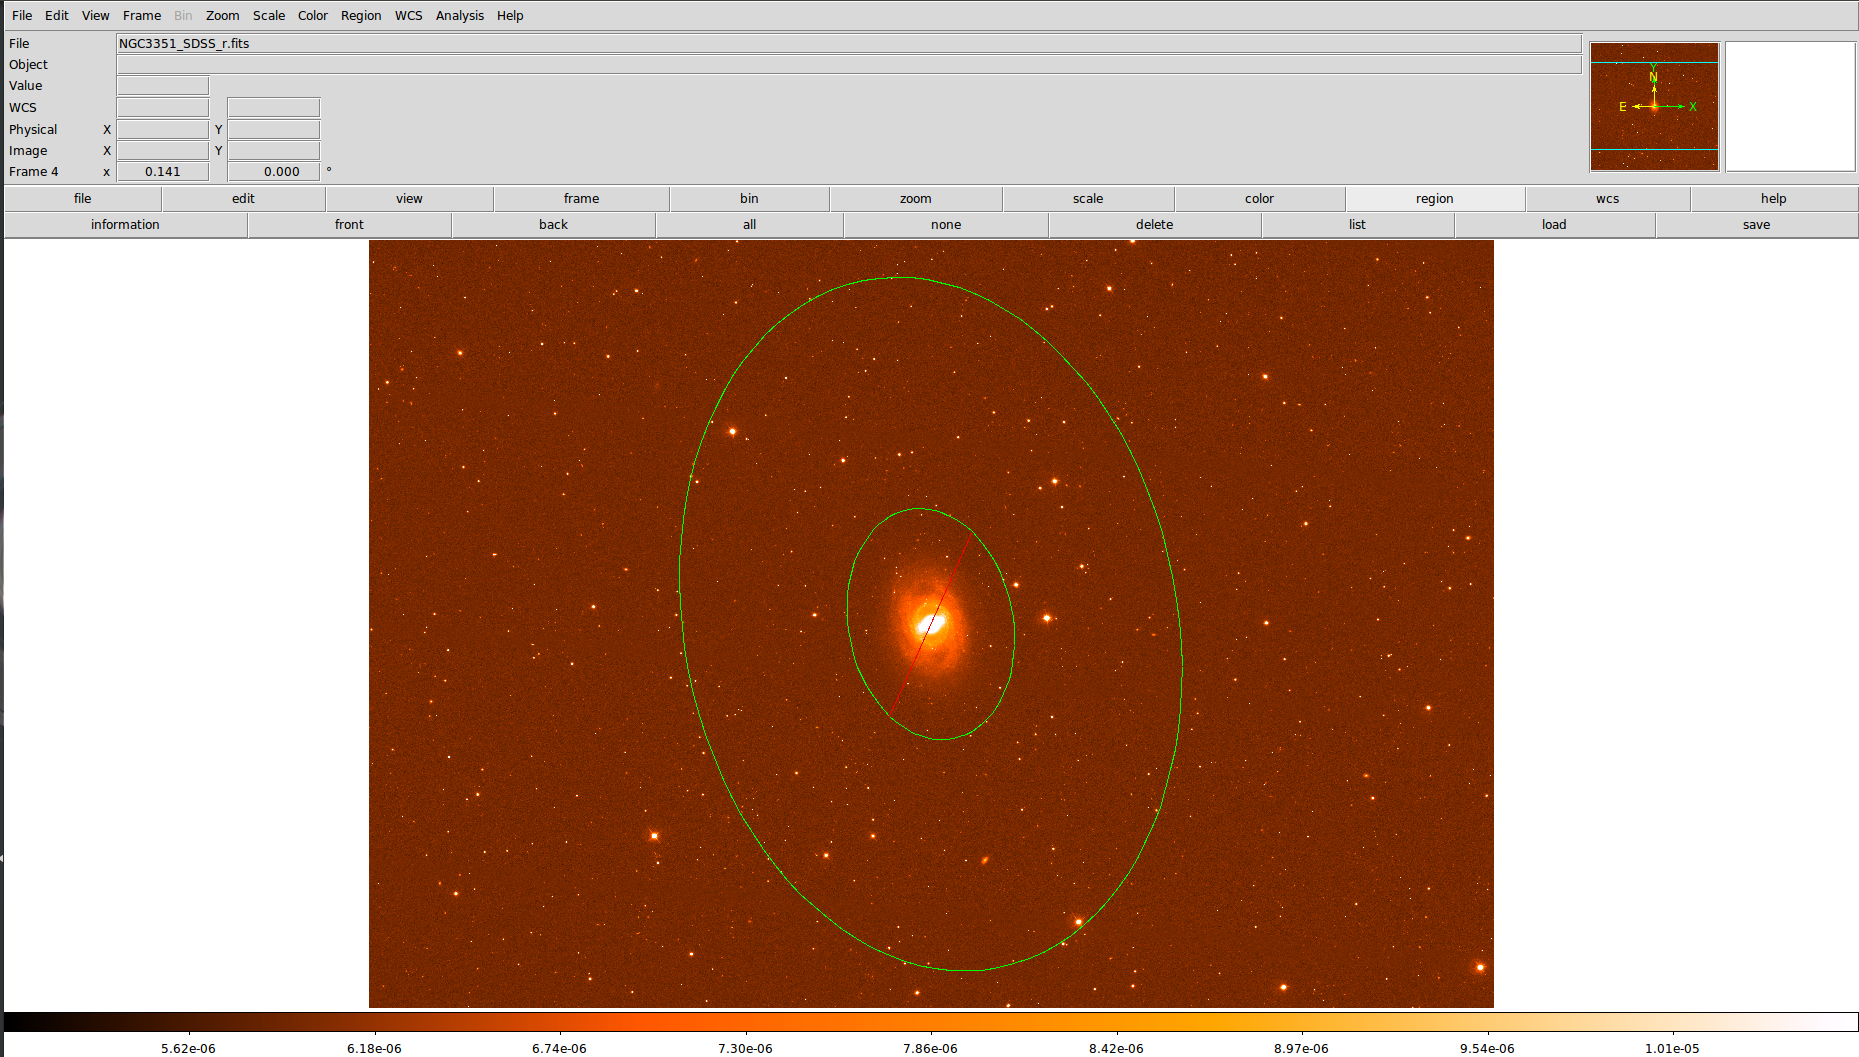
\includegraphics[width=0.7\textwidth]{figures/sky_sub_annulus.png}
\end{center}

Make sure that the inner annulus covers the whole galaxy 
and enough sky to estimate the background noise. If you think that something is wrong stop the program when the plot window is in display, by typing "Ctrl + c" in the terminal. Change the ellipse sizes by decreasing or increasing the annulus factors and re-run the above command. PTS will "know" that you stopped at the sky subtraction step, and will resume from there. If you are not satisfied with the sky subtraction results, you can just delete the files created in the 
"prep/Band\_Name" directory and re-run the sky subtraction step. Delete the following files:

\begin{itemize}
	\item The "sky/" directory
	\item "sky\_subtracted.fits"
	\item "with\_errormaps.fits"
	\item "result.fits"
\end{itemize}

The final image for each band is named "result.fits". When you finish the data preparation stage for each image, just re-run:\\

\textbf{\$ pts prepare\_data}\\

The reason to do that is to auto check that you prepared all images and to add the path of each "Band\_Name/result.fits" to the file called, "dataset.dat".\\

In the following table some of the most important options for the "prepare\_data" command are given.

\begin{table*}[h]
 \begin{center}
 \scalebox{1.0}{
 \begin{tabular}{|l|p{20em}|l|}
 \hline
 \multicolumn{2}{ |c| }{\textbf{prepare\_data}} \\
 \hline
 -{}-aperture\_galaxy\_region\_factor         &default value: 1.5 \\
 \hline
 -{}-sky\_estimation\_method                  &default method: photutils [mean, median, polynomial] \\
 \hline
 -{}-sky\_interpolation\_method$^*$           &default method: polynomial [mean, median, idw] \\
 \hline
 -{}-noise\_interpolation\_method$^*$         &default method: idw [mean, median, polynomial] \\
 \hline
 -{}-sky\_photutils\_polynomial\_order        &default value: 3 \\
 \hline
 -{}-annulus\_inner\_factor                   &default value: 1.2 \\
 \hline
 -{}-annulus\_outer\_factor                   &default value: 4.0 \\
 \hline
 -{}-saturation\_expansion\_factor            &default value: 1.5 \\
 \hline
 -{}-stars\_expansion\_factor                 &default value: 2.0 \\
 \hline
 -{}-interactive\_sky                         &run the sky subtraction in interactive mode \\
 \hline
 \end{tabular}}
 \end{center}
 \caption{*The interpolation methods are used only when you choose photutils as the sky\_estimation\_method.}
\end{table*}

The last command you need to run is the following:\\

\textbf{\$ pts inspect\_preparation -{}-debug}\\

This command will inspect the quality of your image detection. You can check the images in the directory "inspection/inspect\_preparation".\\

\begin{center}
\textbf{CONTINUED IN PART IV...}
\end{center}

\part{Getting More Results}

On this stage, we will do some data processing that will play significant role in later stages of the modeling and map making. First, we decompose the galaxy 
into bulge and disk by using SKIRT. SKIRT will simulate the bulge and the disk based on the data from the S4G database. Thus, before you run the command, make sure that you have installed SKIRT\footnote{\href{http://www.skirt.ugent.be/skirt/\_install\_unix.html}{http://www.skirt.ugent.be/skirt/\_install\_unix.html}}(v8.0) on your local PC.\\

\textbf{\$ pts decompose -{}-debug}\\ 

This command will decompose the bulge from the disk and will convolve the bulge to the IRAC I1 image.\\

Next will truncate the image based on the primary galaxy region. The command is:\\

\textbf{\$ pts truncate 1.3 -{}-debug}\\ 

The number is a factor multiplied with the primary ellipse region of the galaxy, with 1.3 being the default value. You can modify
the number as you please. You can select 1.0 to get just the primary ellipse of the galaxy or lower values than 1.0, but make sure that the truncation ellipse includes the whole galaxy for all of your images. Check this with ds9 by loading the region file which is created in the directory "truncated/ellipse.reg".

\begin{center}
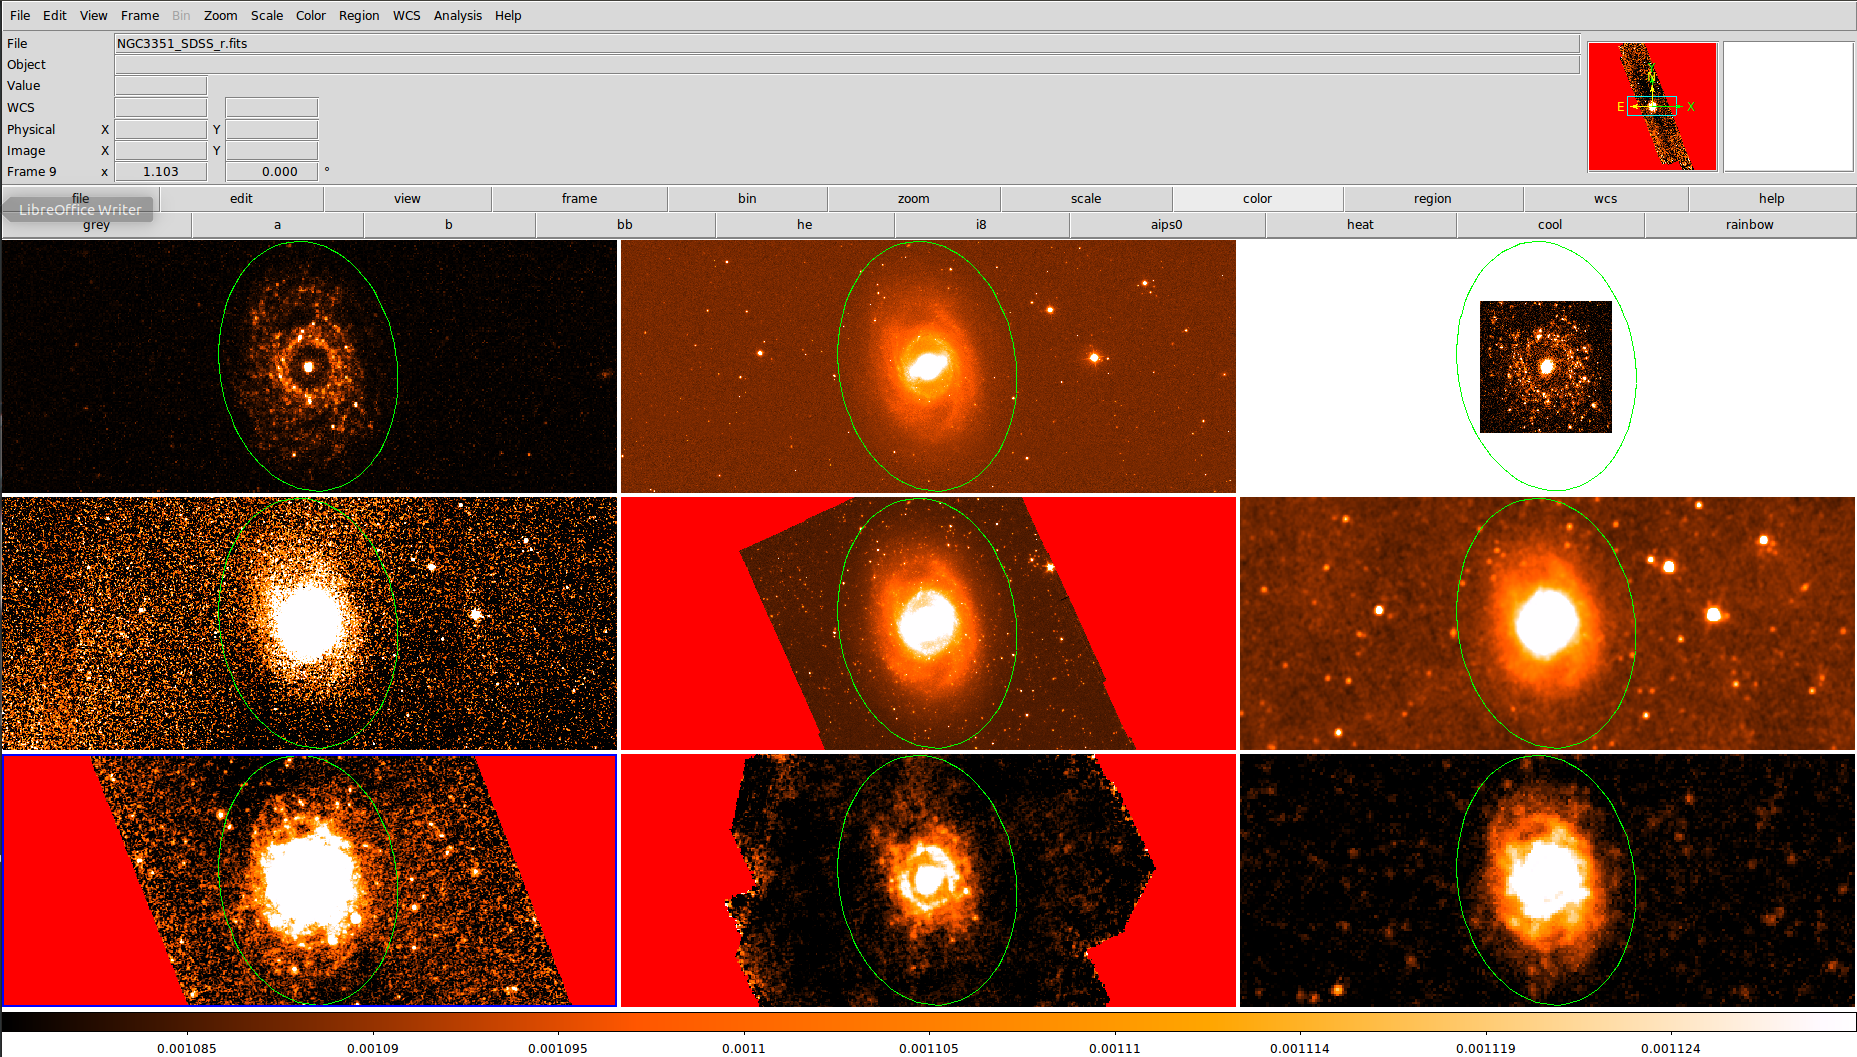
\includegraphics[width=1.0\textwidth]{figures/truncation_ellipse.png}
\end{center}

After this step, we inspect the significance signal levels for each image. Run the following command to create the images of different levels for each band.\\

\textbf{\$ pts generate\_significance\_levels}\\

Go to the directory "truncated/html/significance.html" and click the html file. This will direct you to a web-page.\\

Type then in the terminal:\\

\textbf{\$ pts set\_significance\_levels -{}-debug}\\ 

This command will start a prompt window where you can set the significance levels. Go the significance page and select the best levels by scrolling the bar on top of each band and then type it to the terminal.\\

After you finish with that a file with your choices is created in the directory "truncated/levels.dat". If you are not happy with some of your choices you can just open this file and change the levels from there.\\

Finally, PTS calculates the global fluxes of the images and compares them with the fluxes from DustPedia and from the SEDs that you have downloaded.\\  

\textbf{\$ pts photometry -{}-debug}\\

\begin{figure}[h!]
\begin{subfigure}{.5\textwidth}
  \centering
  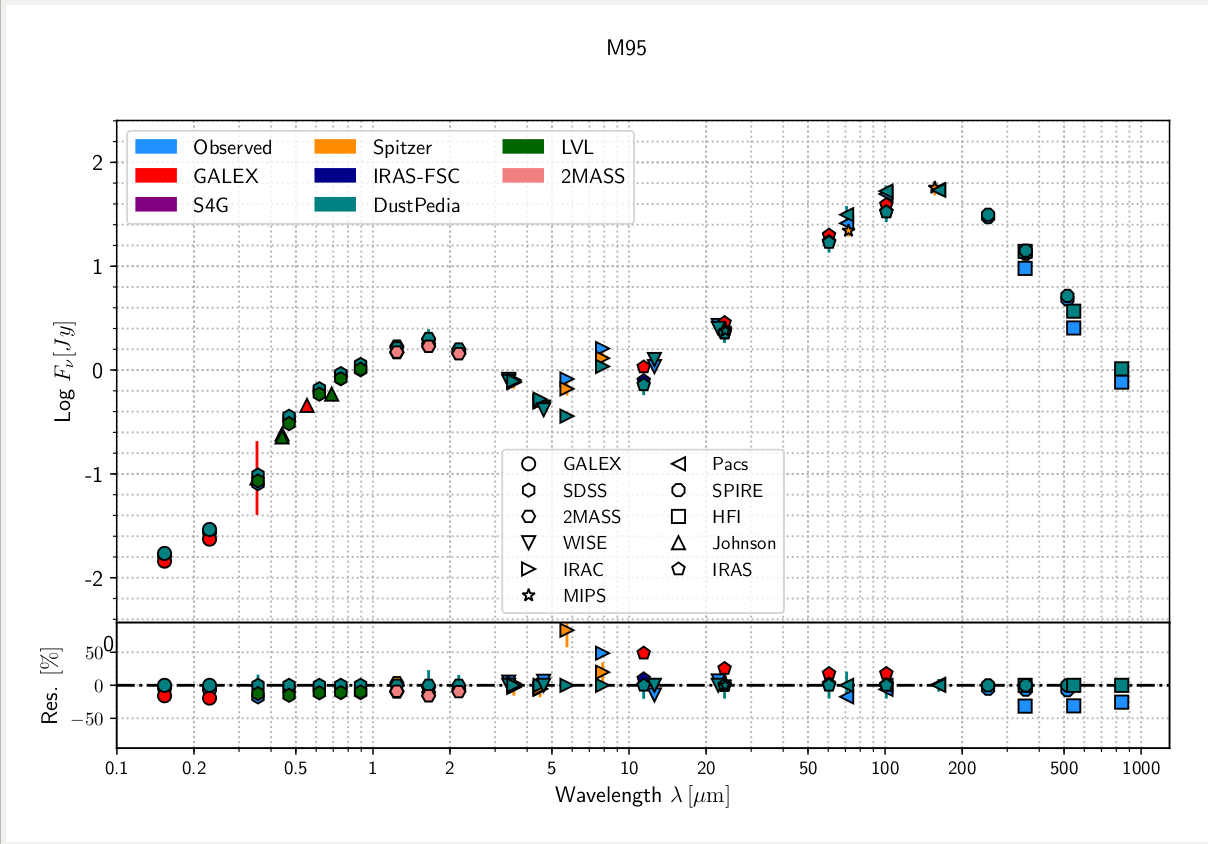
\includegraphics[width=1.0\linewidth]{figures/sed_with_ref.png}
  \caption{SED with references.}
\end{subfigure}%
\begin{subfigure}{.5\textwidth}
  \centering
  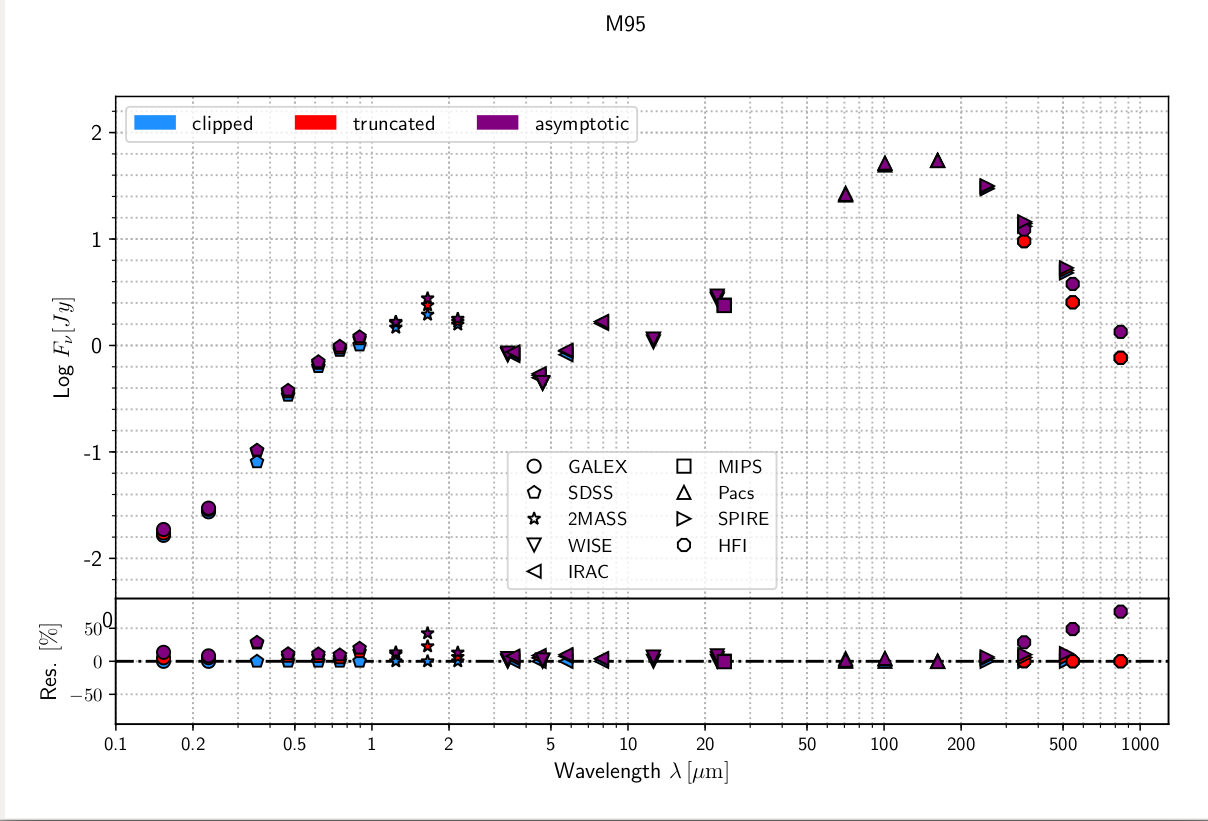
\includegraphics[width=1.0\linewidth]{figures/sed_with_alt.png}
  \caption{SED with alternative photometry estimation.}
\end{subfigure}
%\caption{plots of....}
\end{figure}

This command will compute the global flux for each image, ignoring all pixels that exist outside of the the truncation ellipse (truncated images). It will also compute the fluxes based on the signal-to-noise levels that you selected (clipped images). Finally, it will plot the SEDs in the "phot/" directory, comparing the two photometry estimation methods with SEDs from the literature.\\

\begin{center}
\textbf{CONTINUED IN PART V...}
\end{center}

\part{Creating the Maps}

This part is actually very straightforward just execute the following command in sequence and you will not have any problem. These commands will create the necessary maps that are needed for the SKIRT simulations, in the "maps/raw/" directory.\\

\textbf{\$ pts make\_colours\_maps -{}-debug}\\

\textbf{\$ pts make\_ssfr\_maps -{}-debug}\\

\textbf{\$ pts make\_tir\_maps -{}-debug}\\

\textbf{\$ pts make\_attenuation\_maps -{}-not\_checks cortese -{}-tir\_methods multi -{}-debug}\\

This command will create the attenuation maps based on the calibrations of Cortese et al 2013. Also -{}-tir\_methods multi is used, so that the maps of attenuation would have as many bands as possible.\\

Then by executing the following sequence of commands, you will create the maps where the different components of a galaxy were assumed to be, like the old stellar populations, the young \& ionizing stellar populations and the dust.\\

\textbf{\$ pts make\_old\_stellar\_maps -{}-debug}\\

\textbf{\$ pts make\_dust\_map -{}-debug}\\

\textbf{\$ pts make\_young\_stellar\_maps -{}-not\_use\_buat -{}-debug}\\

\textbf{\$ pts make\_ionizing\_stellar\_maps -{}-debug}\\

You can plot each one of the created maps by typing:\\

\textbf{\$ pts plot\_maps x}\\
 
Where you can replace \textbf{x} with old, dust, young or ionizing.\\

\textbf{\$ pts select\_component\_maps -{}-auto}\\ 

This command will select the best maps for you and will crate a file with the paths of these maps in the directory "maps/components/selection\_0.dat". Then generate the clip maps page so that you could select the significance levels of your component maps.\\

\textbf{\$ pts generate\_clip\_maps\_page}\\

An html file will be created in the "maps/html/clip.html" directory. Click the file and execute the following command so that you can select the levels.\\

\textbf{\$ pts make\_component\_maps -{}-debug}\\ 

This command sets the significance levels of your component maps and also makes your maps smoother, by replacing all negative, nan and inf values and then interpolates the bad pixels around your galaxy. This part might take some time before it's finished, depends on your image values.\\

To visualize the maps type:\\

\textbf{\$ pts plot\_component\_maps}

\begin{center}
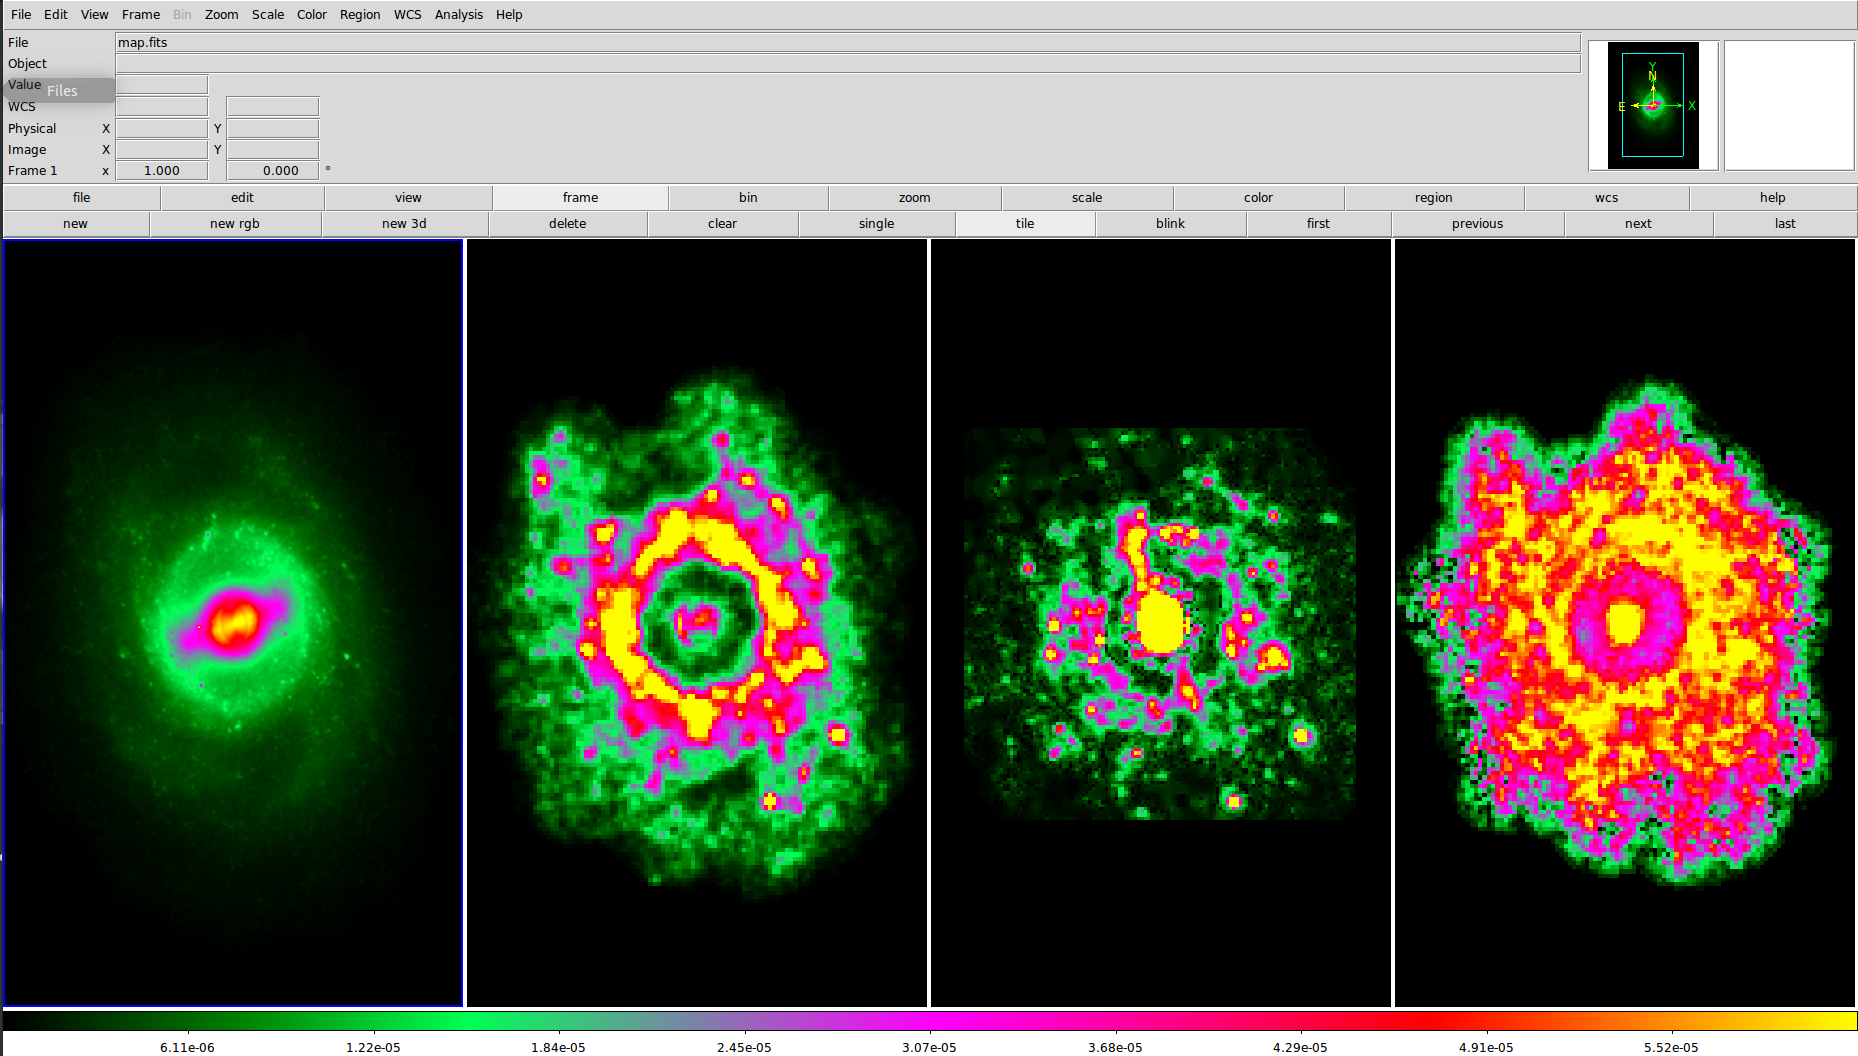
\includegraphics[width=1.0\textwidth]{figures/component_maps.png}
\end{center}

\begin{center}
\textbf{CONTINUED IN PART VII...}
\end{center}

\part{Building Your Galaxy Model}

\textbf{\$ pts build\_model\_galaxy}:

\textbf{\$ pts generate\_representations}:

\textbf{\$ pts configure\_fit}:

\textbf{\$ pts initialize\_fit\_galaxy}:

\textbf{\$ pts explore}:

\begin{center}
\textbf{CONTINUED IN PART VIII...}
\end{center}

% MANAGING
\part{Managing your simulations}

As soon as your initial galaxy models are being simulated with SKIRT on one or more remote machines, you can track their progress (and much more) with the following command:\\

\textbf{\$ pts generation\_status [generation\_name]}\\

The generation name can be obtained from the name of the generation directory in the fitting run's "generations/" directory, or by using the command:\\

\textbf{\$ pts generations},\\

which gives an overview of all the current generations (for different fitting runs in the case there are multiple):

\begin{center}
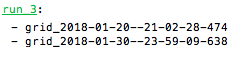
\includegraphics[width=0.4\textwidth]{figures/generations.png}
\end{center}

The status of the generation will be shown as follows:

\begin{center}
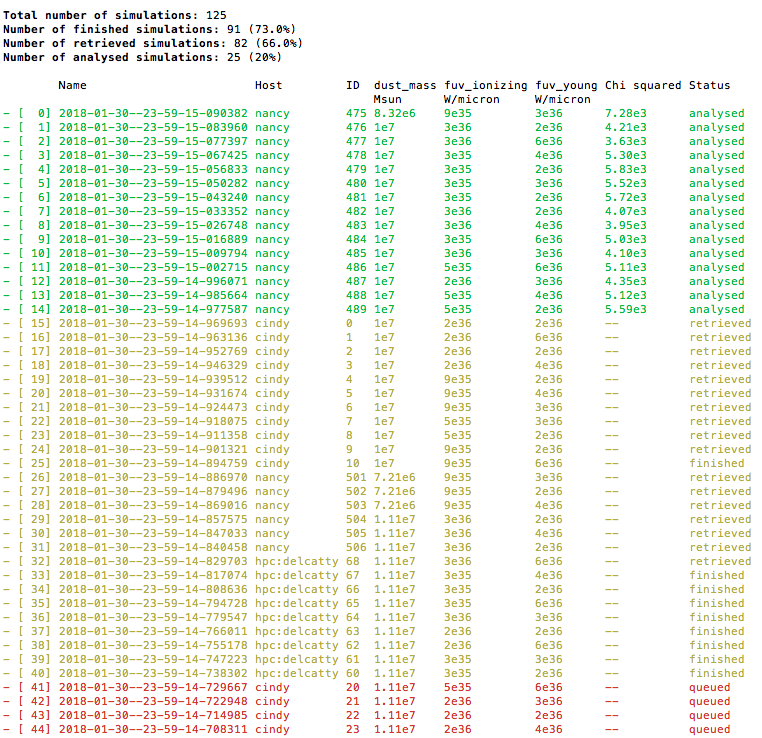
\includegraphics[width=\textwidth]{figures/generation_status.png}
\end{center}

For simulations that are currently running, the current simulation phase and progress will be shown as well under the column "status".\\

When you add the option \textbf{-{}-offline}, no connection to the remotes will be attempted to be made, which means you will get the overview of your simulations quicker. However, the status of simulations that were still queued or running will obviously not be able to be updated. Therefore, the status of these simulations will show as "unknown".

\begin{center}
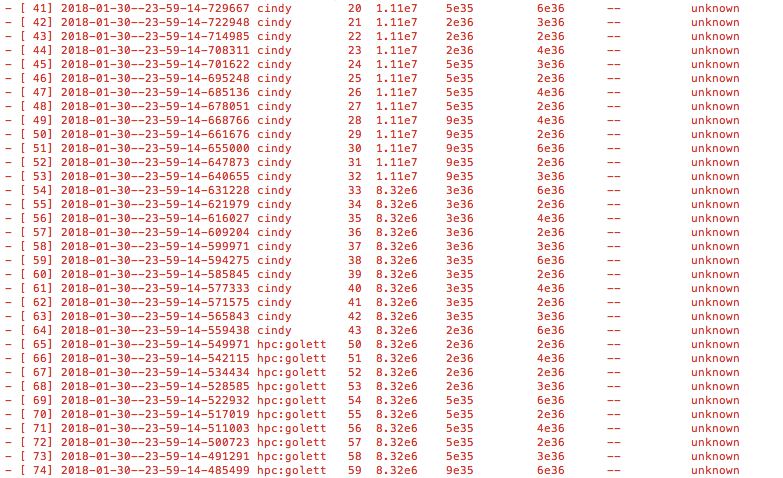
\includegraphics[width=\textwidth]{figures/status_unknown.png}
\end{center}

You can, however, still see the host, the unique simulation ID, and the parameter values for the "unknown" simulations, as for any other simulation in the batch.\\

The functionality of the \textbf{generation\_status} command doesn't end there. More even, it becomes your primary hub to manage all of your simulations, i.e. retrieve and analyze them, move them from one remote host to another, stop and relaunch simulations, view the output, and much more. This is because the \textbf{generation\_status} uses the \texttt{SimulationManager} class under the hood, which can also be invoked freely with the \\

\textbf{\$ pts manage [assignment]}\\

command, passing the filename of the simulation assignment scheme. For each modeling generation that is launched with \textbf{explore}, such an assignment scheme is saved in the generation directory. It stores which simulation (by name) is assigned to which remote host and which unique ID is given to each simulation. Using \textbf{\$ pts generation\_status} is more convenient than using \textbf{\$ pts manage} however, since the former can automatically pass its own assignment scheme, as well as a lot of other information (e.g. the data of which parameter values correspond to which simulation, which enables this info to be shown in the columns as seen above).\\

By adding the \textbf{-{}-extra} option, it is possible to show more information about each simulation. The argument of this option is a sequence of strings denoting which extra information needs to be displayed. Choices include 'screen', 'job', 'disk', 'runtime', and 'memory'. Adding all of these columns to the status output as follows:\\

\textbf{\$ pts generation\_status [generation\_name] -{}-extra screen,job,disk,runtime,memory}\\

gives the following output:

\begin{center}
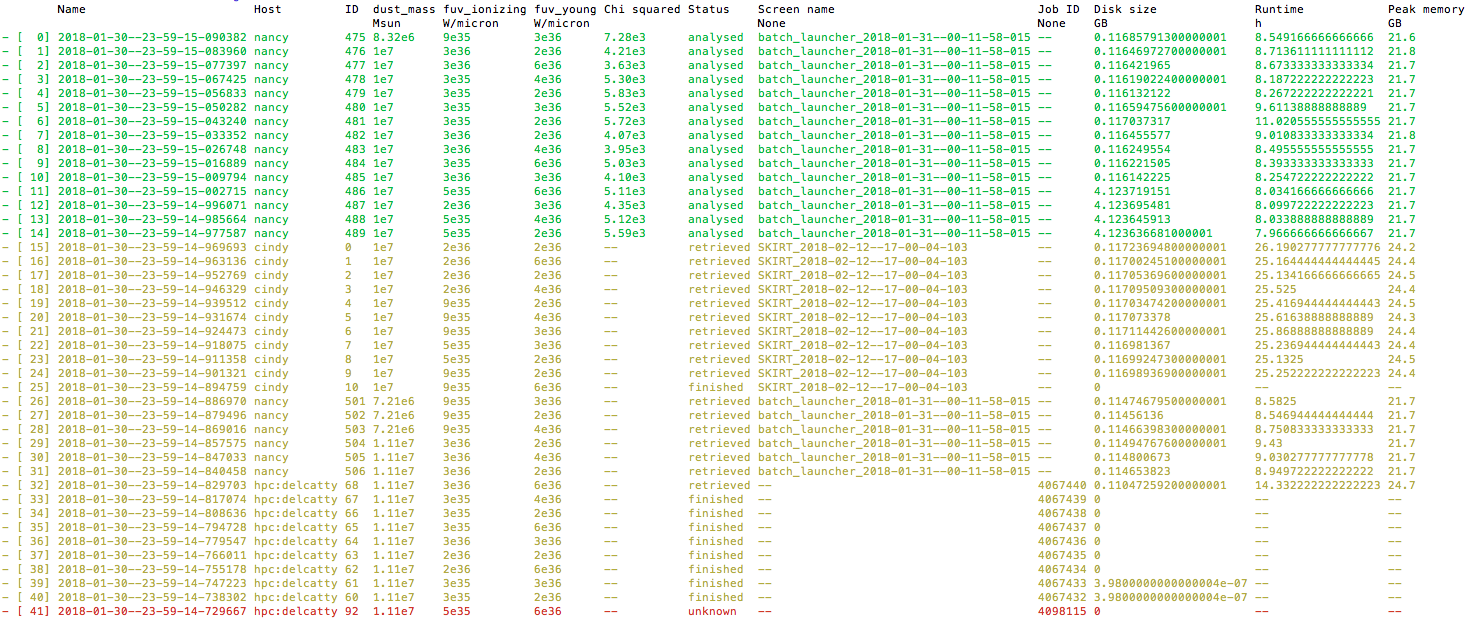
\includegraphics[width=\textwidth]{figures/status_extra.png}
\end{center}

For each extra parameter, a column is displayed. The specified column names respectively display the name of the screen session in which the simulation is launched, the ID of the job associated with the simulation (on systems with a job scheduling platform), the total size of the output files of the simulation, the total runtime of the simulation, and the peak memory consumption.\\

The real interesting feature of the simulation manager is the interactive mode, which allows for many inspections, manipulations and analyses to be executed for specific simulations. The interactive mode is invoked by simply adding \textbf{-{}-interactive} to the \textbf{generation\_status} command, which can be combined with any of the other command-line options. The status of the simulations is shown as otherwise, however hereafter a prompt is shown, indicating that the interactive mode is entered:

\begin{center}
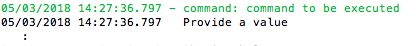
\includegraphics[width=0.5\textwidth]{figures/interactive.png}
\end{center}

There are numerous commands that can be entered into this prompt. A complete list is shown with the "help" command, with an output as shown below (not all command are shown).

\begin{center}
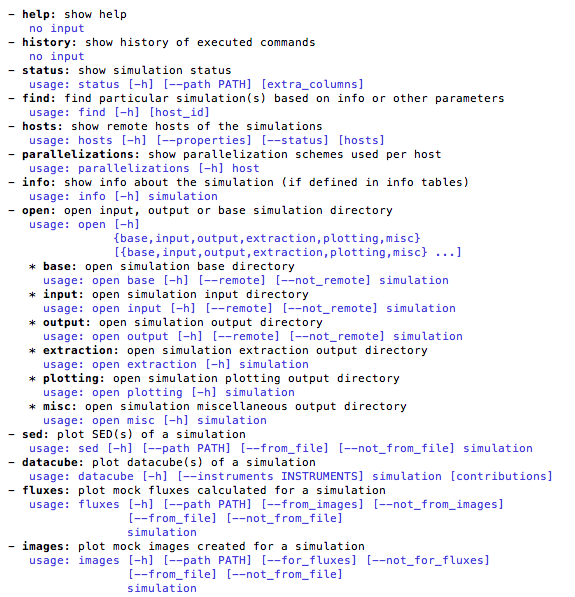
\includegraphics[width=0.8\textwidth]{figures/help.png}
\end{center}

For each command, the usage (expected and optional input) is shown in blue. A brief description is also provided for each command. Some commands don't require input, others operate on the name or index of a simulation, others take a list of simulation indices, others will take the name of a remote host, etc. Which input is expected can be inferred from the usage string, or a more detailed description can be obtained for a certain command by entering \textbf{[command] -{}-help} in the prompt. For example:\\

\textbf{: analyse -{}-help} \\

will display the following output:

\begin{center}
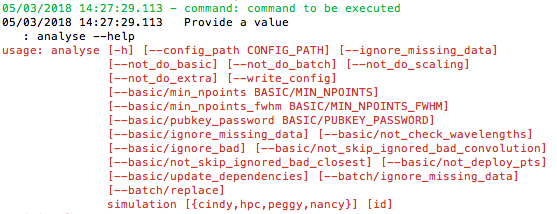
\includegraphics[width=0.9\textwidth]{figures/help_analyse1.png}
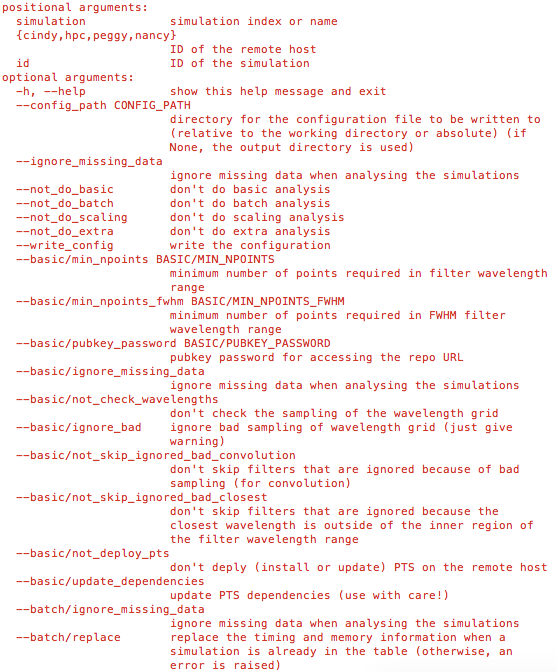
\includegraphics[width=0.9\textwidth]{figures/help_analyse2.png}
\end{center}

Additionally to the usage string, a description is given for each positional and optional argument. For example, the \textbf{analyse} command accepts the simulation index or name as the first argument. \\

We will now describe some of the most useful commands for managing and following up the simulations associated with a RT modeling generation. The first command is simply \textbf{status}, which shows the simulation status again. This is useful to get the overview and find a particular simulation, without having to scroll to the top after some other commands have been executed. Note that by adding \textbf{-{}-refresh} to the \textbf{status} command, the status info will be updated, while the default is to use the previously queried status. The second command is\\

\textbf{: find}\\

which can be used to find the name(s) of one or more simulations with particular values for the modeling free parameters. The command iterates over the different parameters, and shows the unique values associated with that parameter. When one of those values is selected, the simulations that have that particular value for their parameter will be listed. Choosing particular values for the other parameters narrows this list of simulations down, to just one simulation if all free parameter values are chosen. The output looks as follows:

\begin{center}
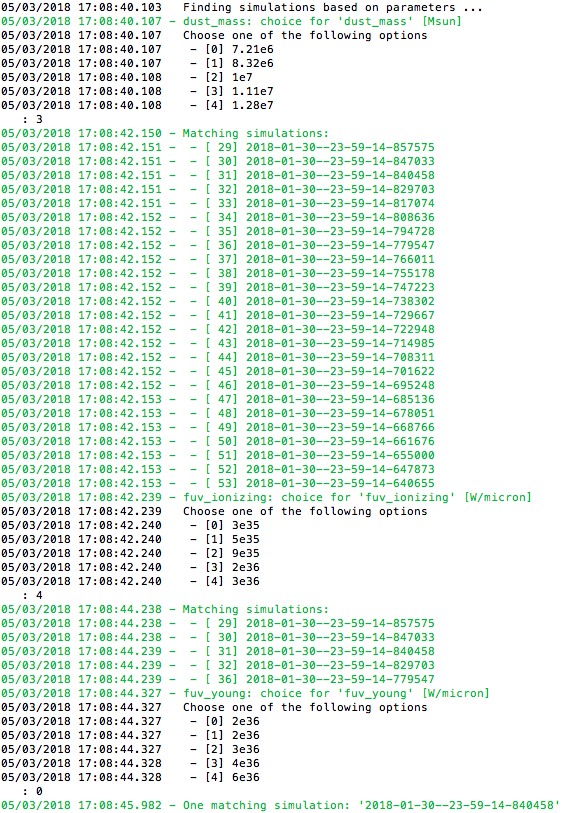
\includegraphics[width=0.8\textwidth]{figures/find_simulation.png}
\end{center}

Using the \textbf{find} command to get the name (or index) of the simulation matching the particular parameter values, the user can effectively apply another command on a simulation, without having to look up the simulation name for those parameters in the output of the \textbf{status} command.\\

When all simulations of the generation were submitted to the same computing host, but other hosts are available, there is a command which can easily speed up the time required for the generation by moving some of the simulations to one or more of these available hosts. This command is \textbf{move}, which can move multiple simulations to the same remote host at the same time. Simulations that can be moved are simulations that are still queued or even already running simulations. These simulations can be moved at any time, or any number of times without problems. So even when simulations are already running on different remotes, the \textbf{move} command can still be used to change the assignment from simulations to hosts. With some attentiveness to the execution time on the different remotes and the number of still queued simulations on each host, the user can balance the load between the remotes just so that the whole of the batch of simulations finishes in the least amount of time. An example use of the \textbf{move} command is the following:\\

\textbf{: move 41-64 hpc:delcatty 16:2:2 --scheduling/walltime 54000 --scheduling/nodes 1}\\

As the first argument, a range of simulation indices is passed (indices can also be separated by commas, or a single index can be given). The next argument is the specification of the host to which to move the simulation(s). The ID or name of the host is usually enough, but if a specific cluster is to be used, the cluster name can also be specified as shown above. As an optional additional argument, the desired parallelization scheme can be passed. A parallelization scheme is an required set of \textbf{[number of cores]:[number of processes]}, and the number of threads per core can be added optionally as \textbf{:[number of threads per core]}. When the parallelization is not specified, PTS will try to determine the most ideal parallelization scheme for your simulations, depending on the available number of CPUs, memory on the remote host. When simulations are moved to a host with a scheduling systems for launching jobs, additional options can be specified such as the walltime (in seconds), which in this case is estimated roughly based on the total runtimes of the already finished simulations of the generation. If not specified, the PTS machinery will also try to estimate the expected walltime based on the remote host and parallelization scheme.\\

When one or multiple simulations are moved to another host, they will not be launched immediately (or even submitted as jobs to the scheduling system), but instead are placed in some sort of a queue. This means that multiple calls of the \textbf{move} command can be executed consecutively, and the simulations for a particular host will be appended to the same queue. Only when no more commands are provided and the interactive mode is left (by simply pressing ENTER in the prompt; without input), the simulations will be submitted to the appropriate hosts. Some output will be shown, where it states the number of simulations in the queue for each host, and lists the parallelization scheme for each of the simulations. Next, the ski files of the simulations will be uploaded to the appropriate hosts:

\begin{center}
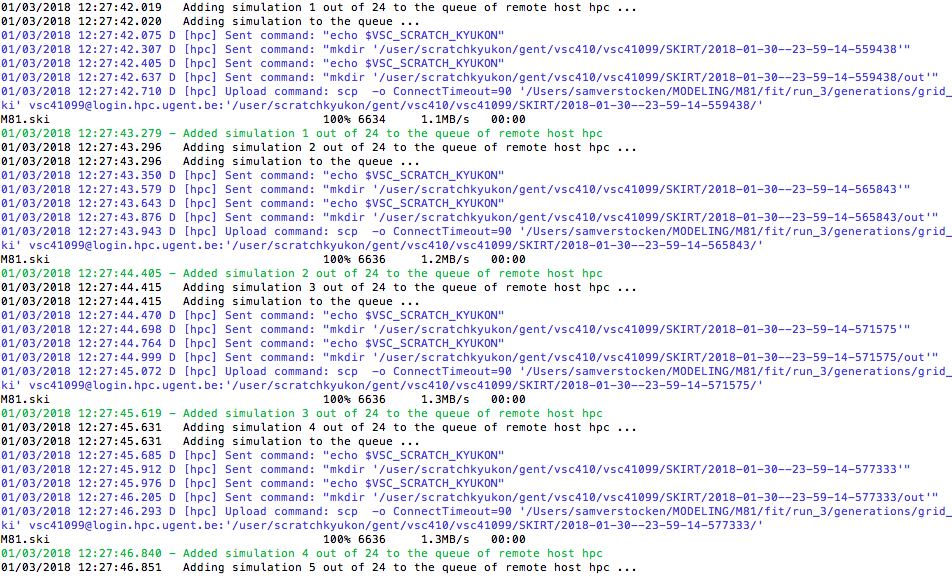
\includegraphics[width=0.9\textwidth]{figures/move_upload_ski.png}
\end{center}

For simulations launched as jobs on a scheduling system, job scripts will be created and also uploaded to the right place on the remote file-system. For other simulations, a shell script will be uploaded per host that executes all the simulations consecutively. Jobs are scheduled, and the ID of the jobs will be shown (in debug mode):

\begin{center}
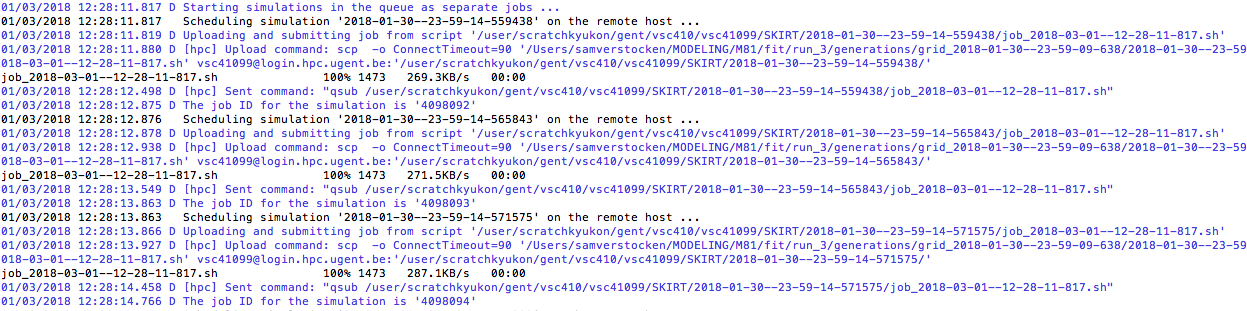
\includegraphics[width=0.9\textwidth]{figures/move_jobs.png}
\end{center}

PTS will automatically check whether the input files (which are the same for each simulation of a generation) are already present on the target remotes (from the initial launch or a previous move). If the input is already present, the files are not uploaded again but the new simulations are referred to the existing input file paths, saving both precious time and disk space.\\

When all simulations are submitted, the simulation assignment scheme (saved in the generation directory) will be updated and saved, and the \textbf{generation\_status} command finishes.\\

With the \textbf{compare} command, the properties of two simulations in the generation can easily be compared. The first argument must be either \textbf{simulation} (to compare simulation settings) or \textbf{analysis} (to compare analysis options). For example, the output of\\

\textbf{: compare simulation 0 1}

looks as follows:

\begin{center}
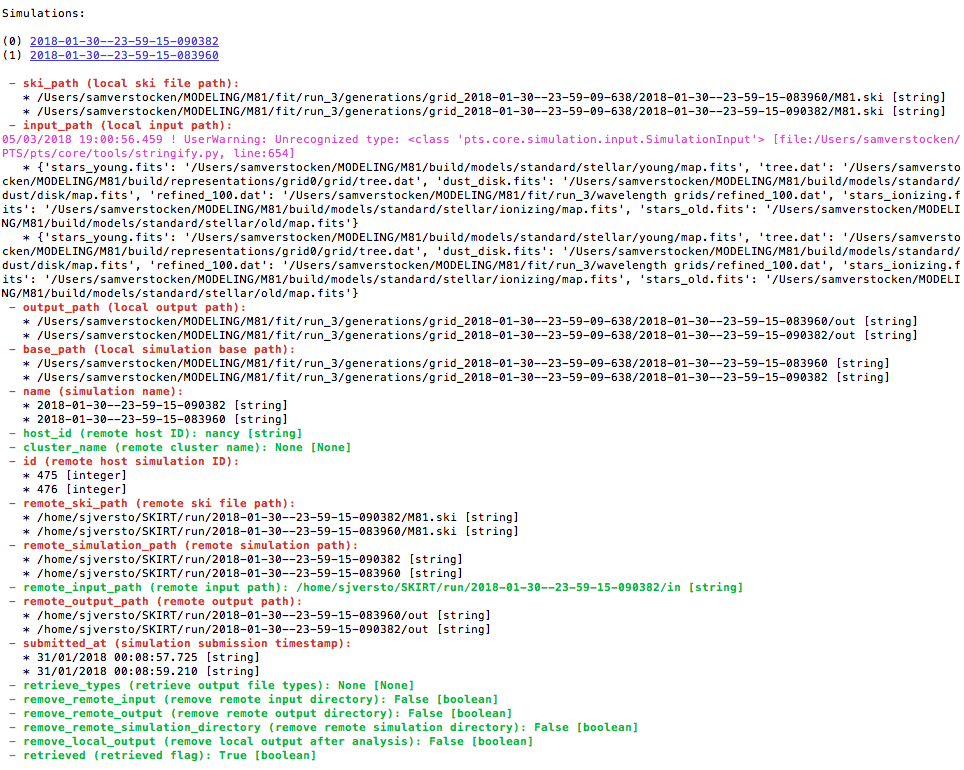
\includegraphics[width=0.9\textwidth]{figures/compare.png}
\end{center}

Because the simulations belong to the same generation, the differences that are listed between both simulations are trivial: they involve just the paths and the things such as the ID and name of the simulation. Also the analysis options are almost identical between simulations, except for paths (not all output is shown):

\begin{center}
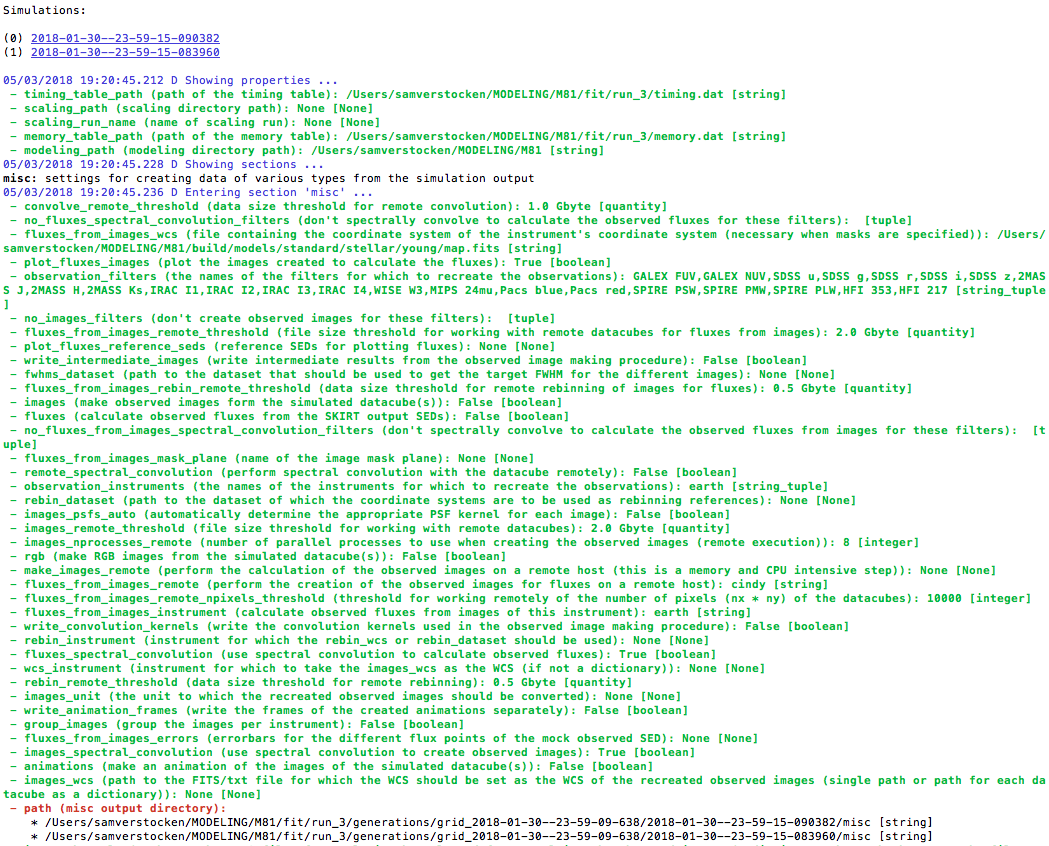
\includegraphics[width=0.9\textwidth]{figures/compare_analysis.png}
\end{center}

The \textbf{compare} command, however, is useful for detecting errors in the simulation settings or analysis options for a certain simulation.\\

Related to the \textbf{compare} command, the \textbf{adapt} command can be used to modify (perhaps fix) certain simulation options and analysis settings. As the \textbf{compare} command, it takes either \textbf{simulation} or \textbf{analysis} as the first argument. The next argument is the name or index of the simulation to be modified. Other optional arguments are mostly identical for either the \textbf{simulation} or \textbf{analysis} subcommand, and can be viewed by running \textbf{adapt simulation -{}-help} (or \textbf{adapt analysis -{}-help}). When running\\

\textbf{: adapt analysis [simulation\_index]}\\

the user will be prompted for each analysis option, and can enter a new value if desired. The various options for the command are very useful to filter out only a specific set of settings that need to be adjusted.\\

Also related, the \textbf{settings} and \textbf{analysis} commands show the simulation settings and analysis options of a simulation, respectively. Very similar options can be used to only show a subset of properties.\\

To view the parameter values of a simulation with a certain name (or index), you can use the \textbf{info} command. It will also show you the chi squared value of the simulation if it had already been analysed:

\begin{center}
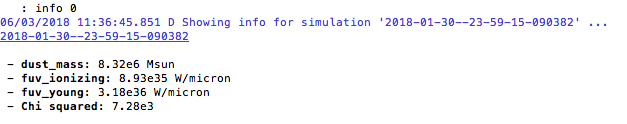
\includegraphics[width=0.9\textwidth]{figures/info.png}
\end{center}

A lot more details about the simulation can be shown with other commands. For example, the \textbf{dust} and \textbf{stellar} commands give an list of all the  dust and stellar components of the model respectively, so calling\\

\textbf{: dust [simulation\_index]}\\

for example gives:

\begin{center}
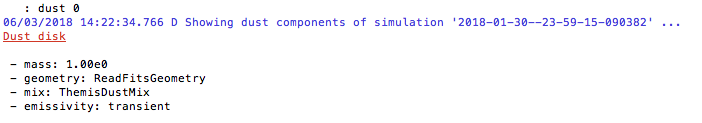
\includegraphics[width=0.9\textwidth]{figures/dust.png}
\end{center}

and\\

\textbf{: stellar [simulation\_index]}\\

gives:

\begin{center}
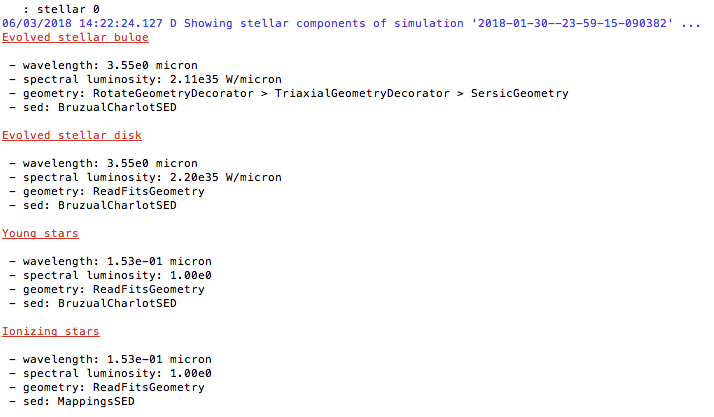
\includegraphics[width=0.9\textwidth]{figures/stellar.png}
\end{center}

The \textbf{instruments} command gives an overview of the instruments that are used for a particular simulations (for the simulations of a generation however, they will be the same for each of them). The output is as follows:

\begin{center}
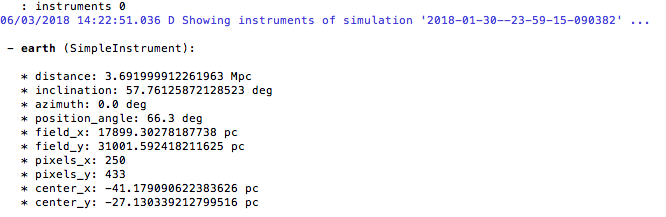
\includegraphics[width=0.9\textwidth]{figures/instruments.png}
\end{center}

A useful, related command is \textbf{normalizations}. It gives an overview of purely the stellar normalization luminosities used for different components at certain wavelengths or filters, and also the total luminosity at that wavelength or filter. When adding \textbf{-{}-flux [flux\_unit]} to this command, the values will also be directly shown in the desired flux (density) unit as well, so for example:\\

\textbf{: normalizations 0 -{}-flux Jy}\\

gives:

\begin{center}
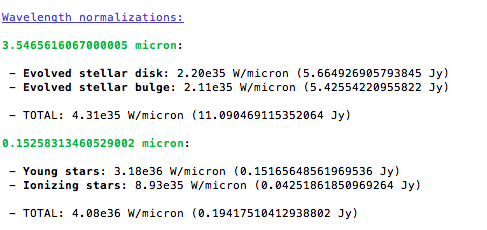
\includegraphics[width=0.6\textwidth]{figures/normalizations.png}
\end{center}

There are also commands to visualize some of the simulation output (when retrieved or analysed). The \textbf{sed} command shows the simulated SED for a particular retrieved simulation (with the observed flux points as a reference), and the \textbf{fluxes} command shows the mock fluxes calculated for an analysed simulation (also with the observed flux points as reference). The \textbf{images} command shows a grid of the mock images created from the simulation output during analysis (only when creating images was enabled in the analysis options). Whenever present, an already created plot file is shown instead of running the plotting procedure again, to save time. Another similar command, \textbf{datacube}, shows the simulated datacube of a simulation in an interactive window. The user can scroll through the wavelength range of the simulation and view each individual frame. The wavelength of the current frame is shown on top of the image.

\begin{center}
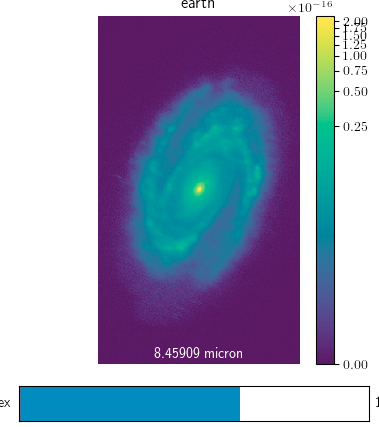
\includegraphics[width=0.6\textwidth]{figures/datacube.png}
\end{center}

Other plotting commands exist, such as the \textbf{plot timeline} command, which visualizes the parallel execution of a particular simulation as a function of time. The command works as follows:\\

\textbf{: plot timeline [simulation\_index]},\\

which shows something like the following:

\begin{center}
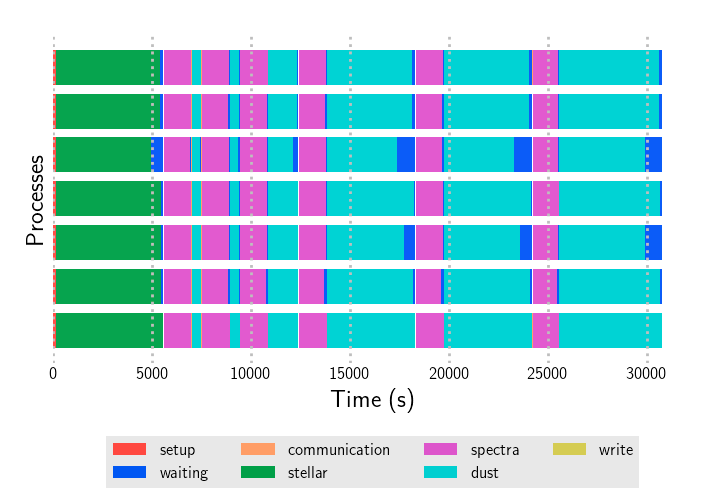
\includegraphics[width=0.9\textwidth]{figures/timeline.png}
\end{center}

To quickly get an overview of all the relevant output files a simulation has produced, simply use:\\

\textbf{: output [simulation\_index]},\\

which will show the names of the output files, categorized:

\begin{center}
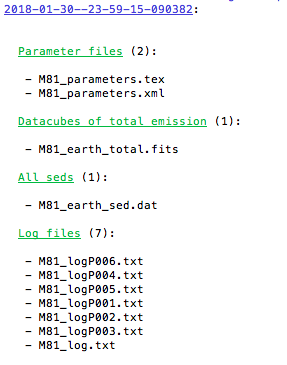
\includegraphics[width=0.5\textwidth]{figures/output.png}
\end{center}

Showing the output works for any finished simulation, even if the simulation has not retrieved yet. This is also the case for the \textbf{log} command, which shows the log output of the simulation. PTS will automatically figure out whether to show the local log file (when the simulation has been retrieved), or to read the log file lines on the remote host (when the simulation has not been retrieved). It also works when the simulation is still running. Adding the \textbf{-{}-summarize} flag shows a more concise version of the log output, that provides a better overview of the different simulation phases. The output of the command:\\

\textbf{: log [simulation\_index] -{}-summarize}\\

is as follows (only a part is shown):

\begin{center}
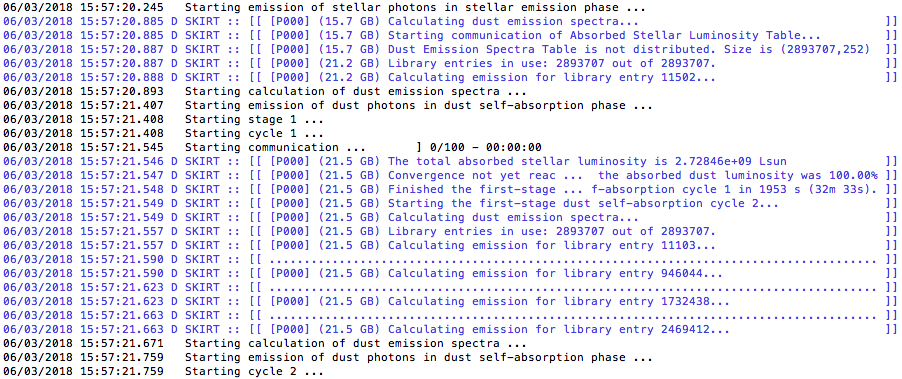
\includegraphics[width=\textwidth]{figures/log_summary.png}
\end{center}

Repetitive SKIRT output is summarized, and intermediate lines printed by PTS mark the beginning and end of the different simulation phases. When the \textbf{log -{}-summarize} command is used on a still running simulation, the output conveniently shows the progress of the current simulation phase:

\begin{center}
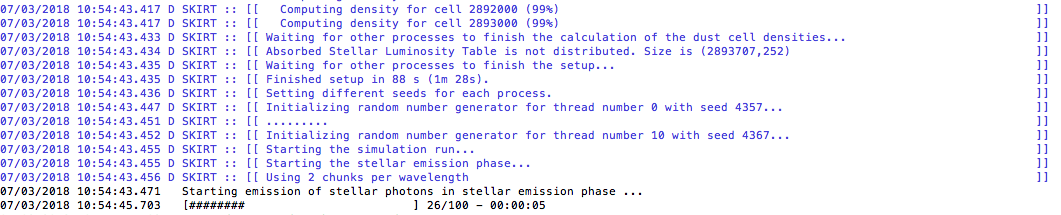
\includegraphics[width=\textwidth]{figures/partial_log.png}
\end{center}

There are also the \textbf{-{}-screen} and \textbf{-{}-job} flags, which can be used to respectively show the screen log output or job output for the simulation instead.\\

Similar to the \textbf{output} command, there are the \textbf{extraction}, \textbf{plotting}, and \textbf{misc} commands, which show the analysis output from the respective analysis steps (if that step has been completed already). The output will look as follows:\\

\textbf{: extraction [simulation\_index]}:\\

\begin{center}
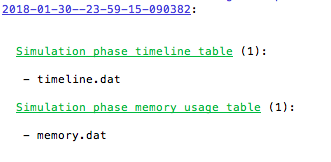
\includegraphics[width=0.5\textwidth]{figures/extraction.png}
\end{center}

\textbf{: plotting [simulation\_index]}:\\

\begin{center}
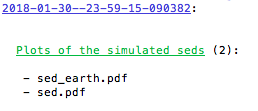
\includegraphics[width=0.4\textwidth]{figures/plotting.png}
\end{center}

\textbf{: misc [simulation\_index]}:\\

\begin{center}
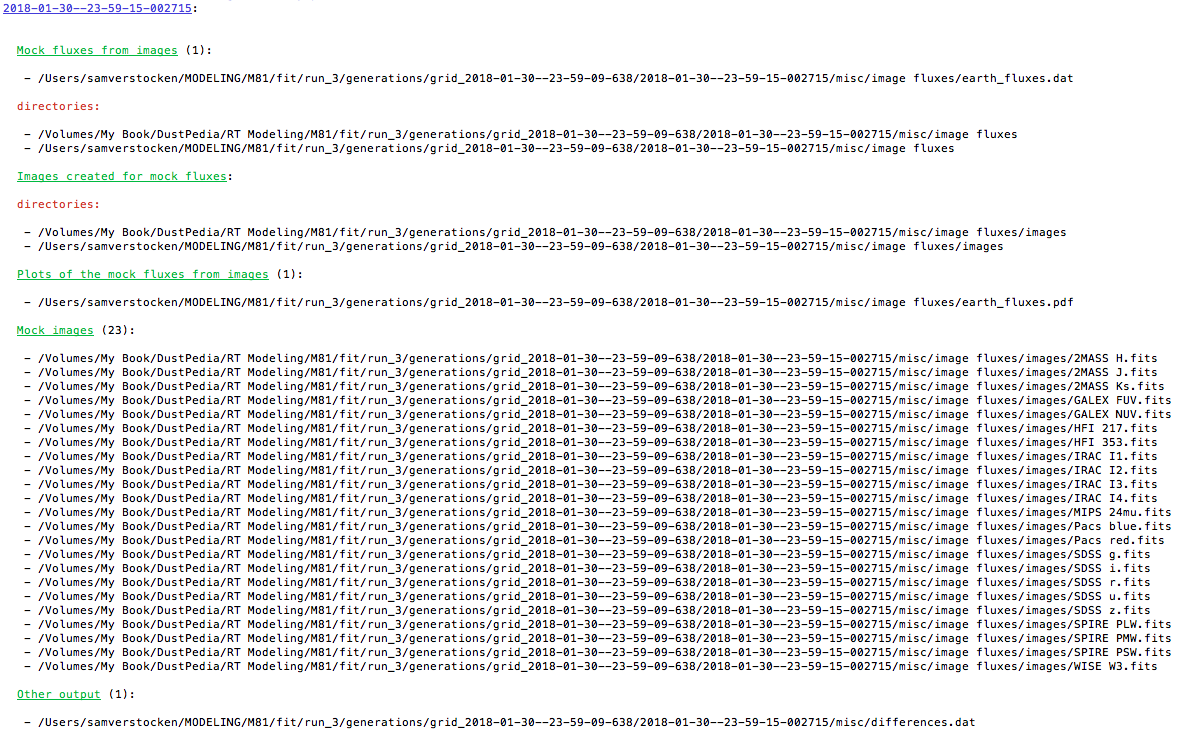
\includegraphics[width=1.\textwidth]{figures/misc.png}
\end{center}

To get more control over whether or not specific simulations are supposed to be running, there are also commands like \textbf{stop} (to stop a running simulation), \textbf{cancel} (to cancel a queued simulation), and \textbf{relaunch}. The latter relaunches a specific simulation to the same remote host, for example after a previously attempted run crashed. The \textbf{remove} and \textbf{clear} commands can be used to completely remove a simulation, as if it never existed (not encouraged!) or to clear the SKIRT output (locally or remotely) or analysis output of a certain simulation.\\

If the status of a particular simulations shows 'crashed' or 'aborted', it may be useful to look into the potential error messages that were printed at the remote host. For this, the \textbf{error} command was created. For example, a part of the simulation status output could show the following:

\begin{center}
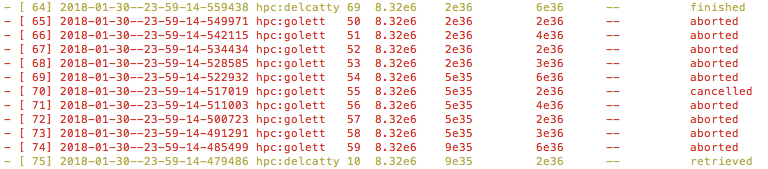
\includegraphics[width=0.8\textwidth]{figures/aborted_cancelled.png}
\end{center}

Looking at the error output of one of these particular simulations is done as follows:\\

\textbf{: error [simulation\_index]},\\

which for example gives the following output:

\begin{center}
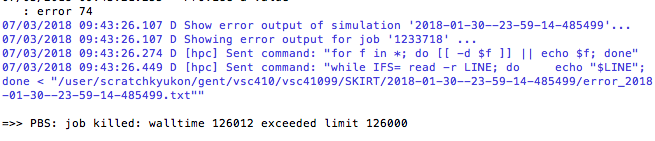
\includegraphics[width=0.7\textwidth]{figures/error_job.png}
\end{center}

In this case, the runtime of the job exceeded the expected walltime of the simulation. In this case, using the \textbf{relaunch} command may be used, with different parallelization and/or scheduling options, or the \textbf{move} command may be used for example if the host (or cluster) seemed unable to run the simulations at all.\\ 

After relaunching or moving the failed simulations, upon rerunning the \textbf{generation\_status} command, the status will show something like:

\begin{center}
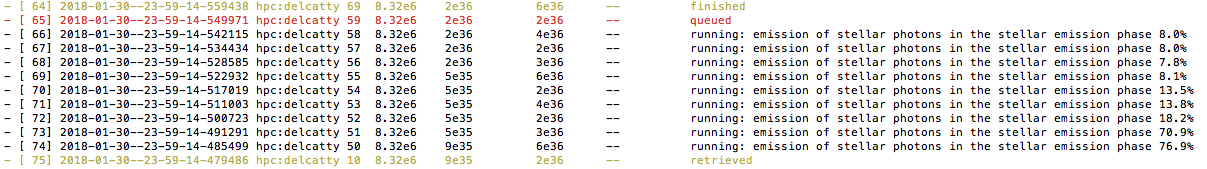
\includegraphics[width=0.8\textwidth]{figures/running_more.png}
\end{center}

All of the commands explained above give a wide variety of tools to manage and inspect simulations, but sometimes it can be useful to quickly open up one of the simulation directories on the file-system. For this, the \textbf{open} command can be used, with as a first argument either \textbf{base}, \textbf{input}, \textbf{output}, \textbf{extraction}, \textbf{plotting}, or \textbf{misc}. Base, input or output directories can be opened either locally or remotely (in which case the appropriate remote host will be mounted). Note that revealing the input files locally (they are scattered across multiple directories) is only supported on MacOS.\\

\part{Analysing the models}

TODO:\\

CACHING\\

ANALYSIS\\

\begin{center}
\textbf{CONTINUED IN PART IX...}
\end{center}

% REFINING
\part{Refining the fitting}

\textbf{\$ pts fit\_sed}:

\textbf{\$ pts show\_best\_simulations}:

\textbf{\$ pts explore run\_number grid host\_name -{}-npoints\_all 5 -{}-auto\_ranges -{}-use\_images -{}-spectral\_convolution -{}-selfabsorption -{}-npackages 5e6 -{}-nprocesses\_remote 7 -{}-nsockets 7 -{}-nwavelengths 100 -{}-test}
\end{document}
